\section{A complete landing in the declared mean-wind case}
\label{sec:wind}
\subsection{Constructing a reference rather than fitting the accident}
The new calculation asks what the stipulated model can construct when conditioned on the report's rounded mean wind. It jointly chooses the approach, flare and touchdown parameters, then applies the unchanged stopping rule. It is not a fit to the recorded accident trajectory and does not impose the report's touchdown state as a terminal target.

The input is wind \emph{from} $070^\circ$ true at 21 kt. The chart's runway bearing of $135^\circ$ magnetic and $1^\circ50'$ west variation give the scenario axis $133^\circ10'$ true. The variation is dated 1990; using it is an explicit convention, not a surveyed 1993 runway registration. In forward/right/up coordinates the resulting constant vector is approximately
\begin{equation}
\mathbf w=(-4.87659,\ 9.64007,\ 0)\ \mathrm{m/s}.
\end{equation}
The forward component is a headwind and the rightward component is crosswind. Appendix~\ref{app:wind} gives the conversion and the case-specific bound.

The synthetic entry position, initial ground track and EAS, threshold conditions, aircraft parameters, twelve-dimensional decision box and original zero-wind reference corridor are retained. Endpoint ground velocities and inverse controls are recalculated for the wind. Consequently this is not a common full-state experiment: fixed EAS and track do not imply fixed ground velocity when wind changes. No nominal calm certificate is reused.

\subsection{The complete approach-to-stop result}
The selected solution uses 41.223 seconds to reach the threshold and 4.142 seconds in flare. It touches down 302.114 metres beyond the usable threshold at 72.490 m/s horizontal ground speed. After the fixed two-second delay, the prescribed deceleration stops it at 2,233.231 metres. The available length is 2,786 metres, leaving 552.769 metres, or 402.769 metres beyond the required reserve.

\begin{table}[H]
\centering\small
\caption{Constructed mean-wind landing. Time is measured from the synthetic entry. These are deterministic model outputs, not a recovered flight or physical prediction interval.}
\begin{tabular}{@{}lrr@{}}
\toprule
Event & Time (s) & Relevant state\\
\midrule
Synthetic entry & 0.000 & 140 m height; 153 kt EAS\\
Threshold crossing & 41.223 & 15.24 m height; 142.281 kt ground speed\\
Touchdown & 45.365 & 302.114 m; 140.909 kt ground speed\\
Braking begins & 47.365 & Fixed delay ends\\
Complete stop & 96.644 & 2,233.231 m; 552.769 m remaining\\
\bottomrule
\end{tabular}
\label{tab:windoutcomes}
\end{table}

\begin{figure}[htbp]
\centering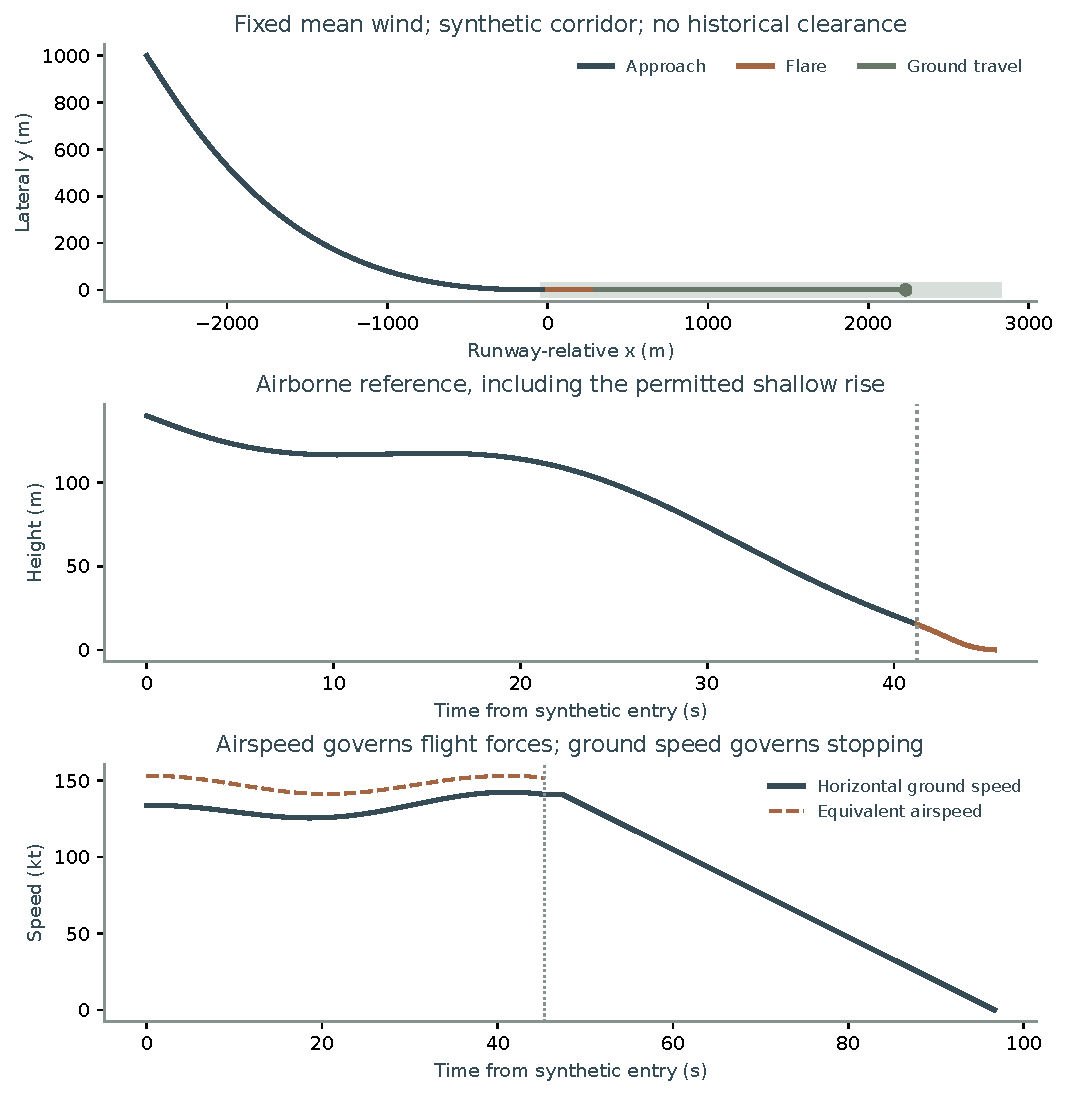
\includegraphics[width=\textwidth]{figures/wind_landing.pdf}
\caption{The new wind-conditioned reference, evaluated from its frozen polynomial coefficients and fixed ground law. The turn, height and speed profiles show a complete landing, including the shallow early rise permitted by the scenario. The ground-speed/EAS difference matters for stopping; ground aerodynamic controls are not extrapolated beyond contact. Coordinates remain synthetic and no historical obstacles enter the solve.}
\label{fig:windlanding}
\end{figure}

Maximum sampled bank is $10.421^\circ$ and maximum bank-angle rate is $2.351^\circ$/s. Touchdown EAS is 151.558 kt, substantially above its 140.909 kt ground speed. The shallow early rise is admissible because monotone descent was not imposed. It must not be hidden by describing the output as a standard approach procedure. Adding that constraint would define a different problem.

\subsection{What the numerical and continuous checks establish}
Four deterministic primary starts succeeded. A denser primary refinement and a secondary effort solve give six retained solver records. On 10,001 exact-rate samples per airborne phase, the selected minimum normalized margin is approximately 0.1527933852. The secondary solution loses approximately $5.22\times10^{-5}$ relative to the retained primary score, within the stipulated $10^{-4}$ tolerance. Agreement among local starts and a small secondary loss are not global optimality proofs.

An independent Newton integration recomputes aerodynamic forces from its integrated state. Its maximum position discrepancy is about $7.3\times10^{-8}$ m and its stop discrepancy about $4.4\times10^{-7}$ m. These values check numerical consistency of the reference and dynamics. They contain no empirical claim about an aircraft's ability to track the curve.

The stronger all-time statement comes from a wind-aware outward-rounded interval calculation at 40 decimal digits. A cover of 376 accepted closed subintervals checks both flight phases, their one-sided join rates, hard inequalities and the exact terminal/ground law. For the declared real-decimal candidate and model it supports
\begin{equation}
\eta_{\mathrm{candidate}}\geq 0.1507934696816132.
\label{eq:windlower}
\end{equation}
This certified lower enclosure is deliberately distinct from the sampled minimum. The lower value reflects enclosure conservatism; it is not an estimated physical safety factor. Its provenance binds the candidate, calculator, checker, configuration and unchanged corridor.

A separate necessary bound, derived from touchdown distance, the minimum permitted ground speed and stopping, gives
\begin{equation}
\eta^*_{\mathrm{wind}}\leq\frac{66656817}{307536544}
\approx0.2167443782.
\label{eq:windupper}
\end{equation}
Here $\eta^*_{\mathrm{wind}}$ denotes the supremum within this fixed scenario family; the zero-wind attainment proof is not silently extended. Combining the two bounds gives
\begin{equation}
0\leq\eta^*_{\mathrm{wind}}-\eta_{\mathrm{candidate}}
\leq0.0659509085084467.
\end{equation}
The right side is rounded upward from the exact rational difference. It is an absolute normalized-score bound, not a percentage performance loss. It is too wide to establish near-optimality or identify the global secondary-effort minimum.

\begin{figure}[htbp]
\centering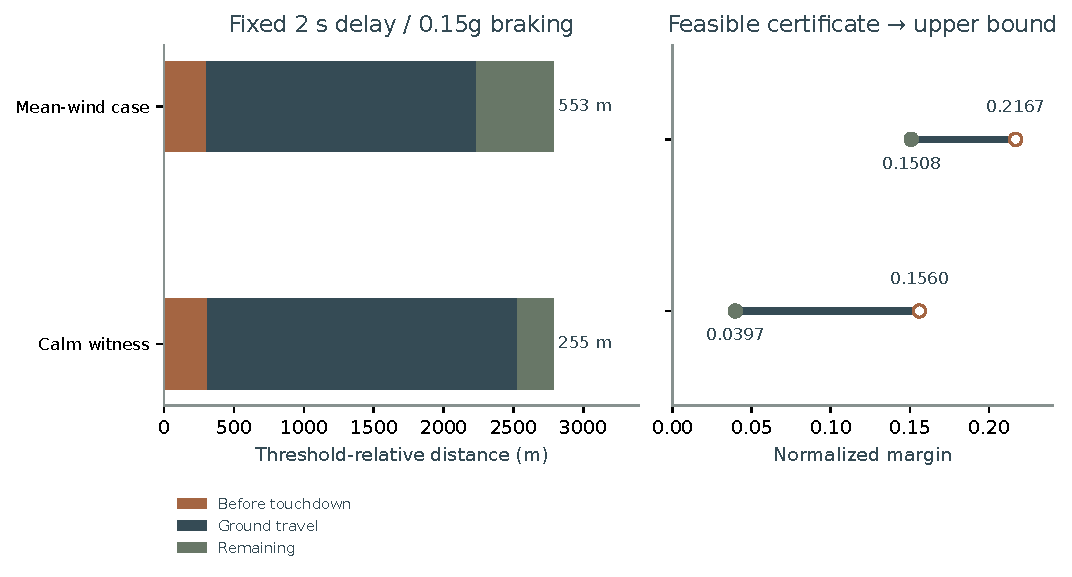
\includegraphics[width=\textwidth]{figures/scenario_comparison.pdf}
\caption{Two declared scenario problems, not a historical treatment comparison. Left: touchdown, ground travel and runway remainder under the same stopping law. Right: surviving certificate-to-upper-bound intervals for the finite-family score. The calm upper endpoint is strict; the mean-wind bound is non-strict. The lower endpoint is a feasible certificate, not the optimizer's proven value. Changing wind also changes endpoint ground velocities and the chosen curve.}
\label{fig:scenariocomparison}
\end{figure}

\subsection{Why the larger runway remainder is not historical superiority}
The new candidate leaves 298.090 metres more than the retained calm witness. In the scalar ground law, 11.378 metres come from its earlier touchdown and 286.712 metres from the difference in speed-dependent ground travel. This is an algebraic decomposition across two outputs, not a causal allocation of the benefit of wind or reoptimization. Both the operating environment and the curve differ, and neither entry state is recovered from CAL605.

The new solve therefore changes the study in a specific way: historical mean-wind information now conditions an explicit complete trajectory with its own certificate. It does not incorporate the observed gust sequence, source-supported historical obstacles, a calibrated wet-runway model or the crew's actual information set. In particular, the CAD finding that actual touchdown was controllable and not causal cannot be overturned by comparing it to this stipulated braking law.

\status{Complete conditional approach/flare/stop reference, independent force replay, all-time model-feasibility certificate and loose family gap bound are available. Historical clearance, physical prediction intervals, global near-optimality and accident-prevention claims remain unestablished.}
